\section{Time plots}

\begin{figure}
\centering
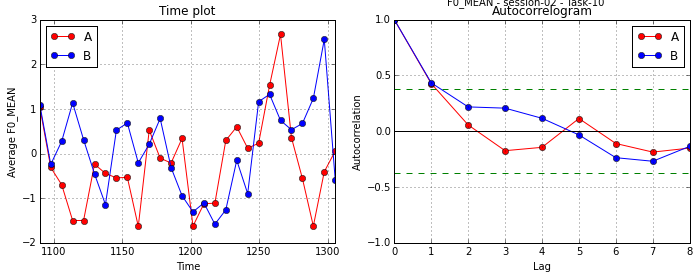
\includegraphics[width=15cm]{images/time_plot_with_autocorrelation.png}
\caption{Time-plot producido por TAMA, junto a su autocorrelación}
\label{fig:time_plot}
\end{figure}

Usando la técnica descripta con las variaciones que consideramos en la anterior sección, generamos dos series de tiempo para cada tarea. Como antes mencionamos, la ventana elegida es de $16''$ con un step de $8''$ lo cual da un overlap del 50\%.

Dada una ventana, puede ocurrir que alguno de los interlocutores no haya hablado, o su interacción haya sido demasiado breve como para medir sus variables a/p. Como ya mencionamos en \ref{sec:tama_modifications}, y a diferencia de \cite{KOU2008.2}, construimos las series sin ese punto, y sin interpolarlo tampoco.

De estas tareas, sólo nos quedamos con aquellas que tengan al menos 5 puntos definidos para cada serie, de manera que tenga sentido poder calcular la correlación cruzada más adelante. Con ésto, no sólo nos interesa la duración de la charla, sino cierta calidad de las series generadas. En \ref{time_series_table} pueden verse las tareas que tuvimos en consideración, a la vez que su duración.

\begin{figure}
\centering

\adjustbox{max width=\textwidth}{\begin{tabular}{lllllllllllll}
\toprule
Task & S-01 & S-02 & S-03 & S-04 & S-05 & S-06 & S-07 & S-08 & S-09 & S-10 & S-11 & S-12 \\
\midrule
01 &         -- &         -- &    149.888 &         -- &         -- &         -- &         -- &         -- &     54.514 &    106.096 &         -- &     56.135 \\
02 &         -- &         -- &         -- &         -- &         -- &         -- &         -- &         -- &     41.711 &     63.837 &         -- &         -- \\
03 &         -- &     51.762 &         -- &     80.737 &     77.977 &     69.260 &     68.489 &     49.607 &         -- &    122.272 &     81.037 &         -- \\
04 &         -- &    187.201 &     93.333 &     76.131 &     79.946 &     99.240 &     84.342 &         -- &     58.020 &    129.621 &     67.977 &     95.292 \\
05 &         -- &         -- &         -- &     86.336 &         -- &    126.759 &    145.849 &     90.742 &     45.773 &    134.206 &         -- &         -- \\
06 &         -- &         -- &         -- &         -- &         -- &    148.218 &     50.672 &     60.281 &     46.165 &     66.762 &     46.773 &     40.200 \\
07 &         -- &     66.024 &         -- &    117.762 &         -- &     72.410 &         -- &     87.702 &     85.900 &    110.675 &     65.758 &         -- \\
08 &         -- &    458.885 &     98.681 &    203.867 &         -- &    188.708 &     59.933 &     48.144 &         -- &    157.442 &         -- &     81.165 \\
09 &         -- &         -- &         -- &     75.551 &    134.247 &     83.045 &    108.786 &         -- &     62.128 &    404.014 &     41.097 &     92.555 \\
10 &     50.131 &    231.392 &    162.895 &    242.588 &         -- &    122.408 &     71.198 &     74.775 &         -- &    356.079 &     69.834 &     92.769 \\
11 &         -- &     74.400 &         -- &     98.634 &     70.189 &         -- &     58.911 &         -- &     72.947 &    104.036 &     59.495 &    101.970 \\
12 &     61.331 &     90.100 &    129.129 &    182.917 &         -- &    130.375 &     75.891 &     57.656 &         -- &    101.661 &         -- &     64.842 \\
13 &     55.146 &    124.095 &    108.196 &    144.193 &    114.720 &         -- &         -- &     83.828 &     94.087 &    174.009 &     84.824 &     91.525 \\
14 &         -- &     75.334 &         -- &         -- &    107.356 &         -- &     52.583 &    144.378 &     75.589 &    108.456 &     91.648 &     98.487 \\
\bottomrule
\end{tabular}
}

\label{time_series_table}
\caption{Tabla de tareas seleccionadas y sus duraciones}
\end{figure}

Los autocorrelogramas de las series bajan rápidamente a cero, un indicio (necesario pero no suficiente) de que las series son estacionarias.

